\documentclass{report}
\usepackage[fontsize=13pt]{scrextend}

\usepackage{my_lab}

\begin{document}

\graphicspath{{figures}}

\MiptLabTitle{4.3.2-B}{Дифракция света на ультразвуковой волне в жидкости}

\begin{document}
\textbf{Цель:} изучение дифракции света на синусоидальной акустической решётке и наблюдение фазовой решётки методом тёмного
поля.

\textbf{Используются в работе:} оптическая скамья, осветитель, два длиннофокусных объектива, кювета с жидкостью, кварцевый излучатель
с микрометрическим винтом, генератор ультразвуковой частоты, линза, вертикальная нить на рейтере, микроскоп.

\section*{Установка}

\begin{figure}[h!]
	\centering
	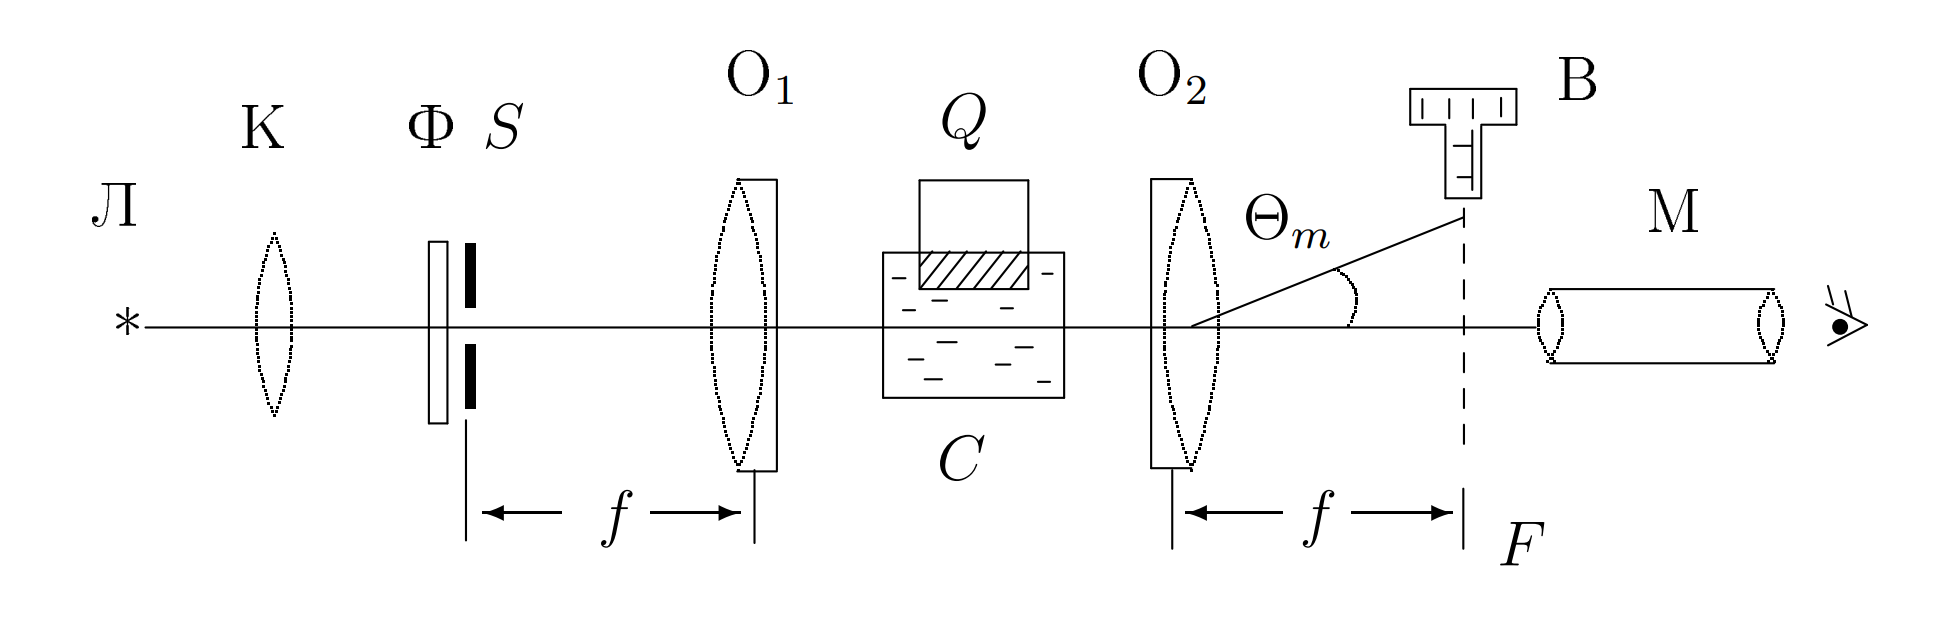
\includegraphics[width=0.9\textwidth]{figures/schema1.png}
	\caption{Схема для наблюдения дифракции на акустической решетке}
	\label{shema1}
\end{figure}
\begin{description}
	\item[Л] -- источник света.
	\item[Ф] -- светофильтр (красный).
	\item[К, $O_1$, $O_2$] -- линзы.
	\item[С] -- емкость с водой.
	\item[Q] -- источник волн.
	\item[B] -- стекло с перемещающим винтом.
	\item[М] -- микроскоп.
\end{description}

Схема установки приведена на рисунке \ref{shema1}. Источник света Л через светофильтр Ф и
конденсор К освещает вертикальную щель $ S $, находящуюся в фокусе объектива $
	O_1 $. После объектива параллельный световой пучок проходит через кювету С
перпендикулярно акустической решетке, и дифракционная картина собирается в
фокальной плоскости объектива $ O_2 $ , наблюдается при помощи микроскопа М.


Измерим положения дифракционных максимумов с помощью микроскопического винта B.

\begin{figure}[H]
	\centering
	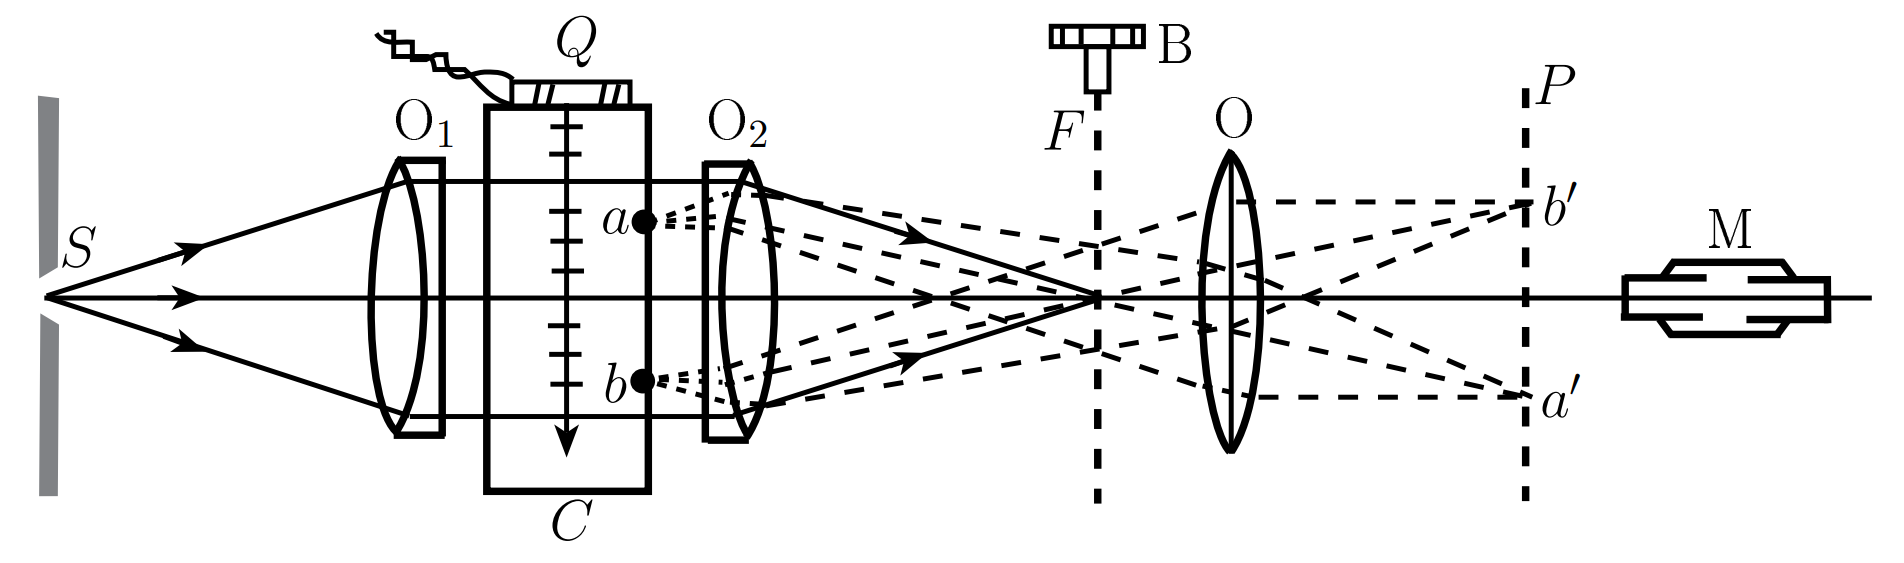
\includegraphics[width=0.9\linewidth]{figures/schema2.png}
\end{figure}

Для наблюдения акустической решетки используется метод темного поля, который
заключается в устранении центрального дифракционного максимума с помощью
непрозрачного экрана.

\begin{figure}[h!]
	\centering
	\begin{minipage}{0.4\textwidth}
		\centering
		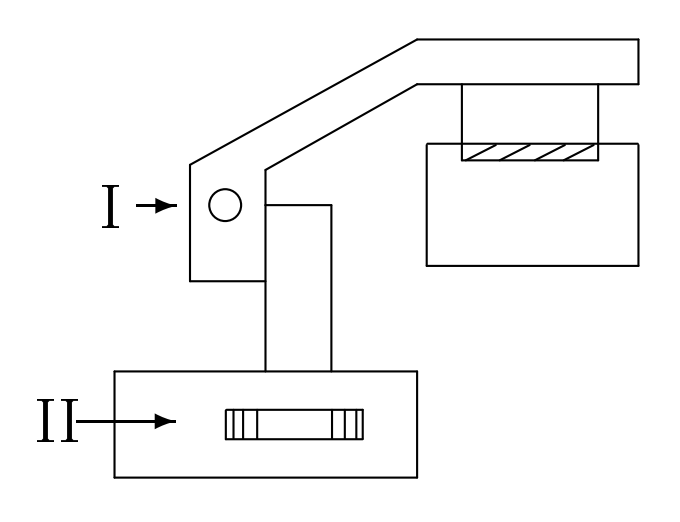
\includegraphics[width=0.9\textwidth]{figures/thing1.png}
		\caption{Устройство для вертикального перемещения излучателя}
	\end{minipage}
	\hspace{1cm}
	\begin{minipage}{0.4\textwidth}
		\centering
		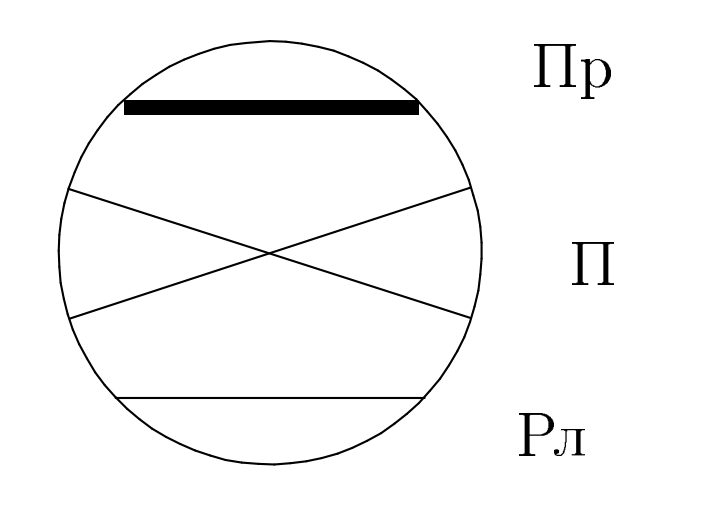
\includegraphics[width=0.9\textwidth]{figures/microscope_fig.png}
		\caption{Проволока, Пр, перекрестие П и реперная линия Рл в плоскости F}
	\end{minipage}
\end{figure}

\section*{Теоретическая часть}

\begin{equation}\label{}
	n = n_0 (1 + m \cos \Omega x)
\end{equation}
$n$ - коэфф. приломления в воде.

\begin{figure}[H]
	\centering
	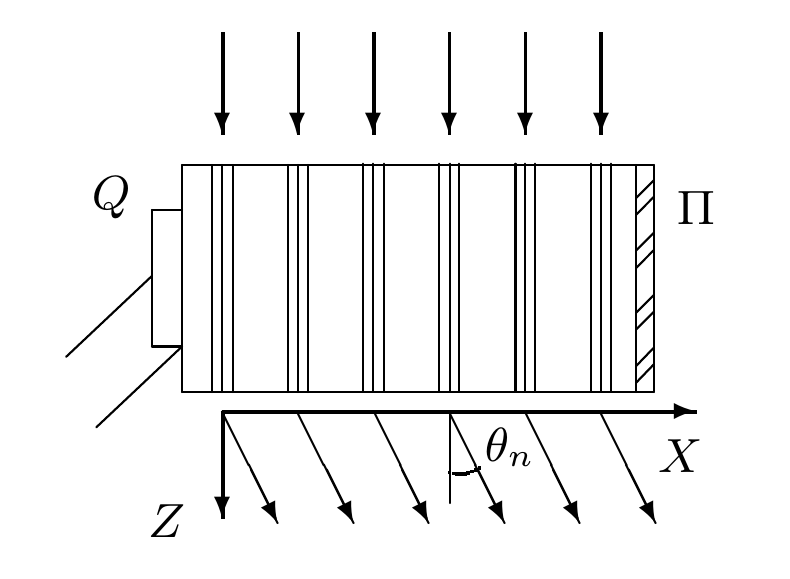
\includegraphics[width=0.7\linewidth]{figures/difraction.png}
	\caption{Эффект дифракции на ультразвуковой волне}
\end{figure}
\\
Фаза колебаний на задней стенке С:
\begin{equation}\label{}
	\phi  = k n L = \phi_0 (1 + m \cos \Omega x)
\end{equation}
$k = \frac{2\pi}{\lambda}$ -- вонновое число.

\begin{equation}\label{}
	\Lambda \sin \theta_m = m \lambda
\end{equation}

\begin{equation}\label{}
	\Lambda = m \lambda F / l_m
\end{equation}

\begin{equation}\label{}
	v = \Lambda \nu
\end{equation}

\section*{Ход работы}
\section{Определение скорости ультразвука по дифракционной картине}
\begin{enumerate}
	\item Соберем схему.
	\item Получим дифракционную картину в микроскопе. \\
	      Для этого включим излучатель. \\
	      Найдем д.к. на частоте $\nu \approx 1 \mega\Hz$. \\
	      Д.к. должна иметь $\pm 7$ максимумов. \\
	      С помощью микроскопа и отметок на стеклышке определим положение
	      дифракционных максимумов по Y. \\
	\item Повторим п. 2 для 4-5 различных частот в интервале $[1, 8] \mega\Hz$. \\
	      Резултаты приведены в таблице.

	      \begin{table}[H]
		      \centering
		      \begin{tabular}{|c|c|c|c|c|c|}
			      \hline
			      $n$            & 1                                     & 2     & 3     & 4    & 5    \\
			      \hline
			      $\nu_n, \mega$ & 1.057                                 & 2.065 & 3.052 & 5.02 & 6.56 \\
			      \hline
			      m              & \multicolumn{5}{c|}{$Y_n,  \micro\m$}                               \\
			      \hline
			      -7             & -310                                  &       &       &      &      \\
			      \hline
			      -6             & -260                                  &       &       &      &      \\
			      \hline
			      -5             & -208                                  &       &       &      &      \\
			      \hline
			      -4             & -200                                  &       &       &      & -110 \\
			      \hline
			      -3             & -170                                  & -110  &       & -70  & -90  \\
			      \hline
			      -2             & -110                                  & -60   & -125  & -50  & -50  \\
			      \hline
			      -1             & -50                                   & -30   & -40   & -20  & -30  \\
			      \hline
			      0              & 0                                     & 0     & 0     & 0    & 0    \\
			      \hline
			      1              & 70                                    & 90    & 70    & 50   & 50   \\
			      \hline
			      2              & 140                                   & 140   & 120   & 70   & 70   \\
			      \hline
			      3              &                                       & 190   & 170   & 120  & 100  \\
			      \hline
		      \end{tabular}
		      \caption{Положения максимумов}
	      \end{table}

	\item Построим графики $Y_n(m)$. \\
	      \begin{figure}[H]
		      \centering
		      \includesvg[width=0.9\linewidth]{figures/Yn(m)-wb.svg}
	      \end{figure}

	      \begin{gather}
		      Y_n(m) = m \lambda f / \Lambda_n \\
		      \alpha_n = \frac{\D Y_n}{\D m} \\
		      \Lambda_n = \frac{\lambda f}{\alpha_n}
	      \end{gather}

	      \begin{table}[H]
		      \centering
		      \begin{tabular}{|c|c|c|c|}
			      \hline
			      $n$ & $\alpha_n, \micro\m$ & $\Lambda_n, \cm$ & $v_n, \frac{\m}{\sec} \cdot 10^3$ \\
			      \hline
			      1   & 48                   & 0.37             & 4                                 \\
			      2   & 51                   & 0.35             & 7                                 \\
			      3   & 58                   & 0.31             & 9                                 \\
			      4   & 31                   & 0.57             & 29                                \\
			      5   & 31                   & 0.58             & 38                                \\
			      \hline
		      \end{tabular}
	      \end{table}

	      В общем, полная ерунда. \\
	      Табличное значение скорости звука в воде:
	      \[
		      v = 1500 \frac{\m}{\sec}
	      \]
\end{enumerate}


\section{Определение скорости ультразвука методом тёмного поля}
Данная часть работы у нас не получилась. \\
Мы смогли сфокусировать микроскоп на калибровочную сетку, но не смогли закрыть
дифракционный максимум проволочкой на стекле. \\

\newpage

\section*{Выводы}
Работа получилась просто ужасно. \\
Хотя бы пронаблюдали дифракцию.

\begin{figure}[H]
	\centering
	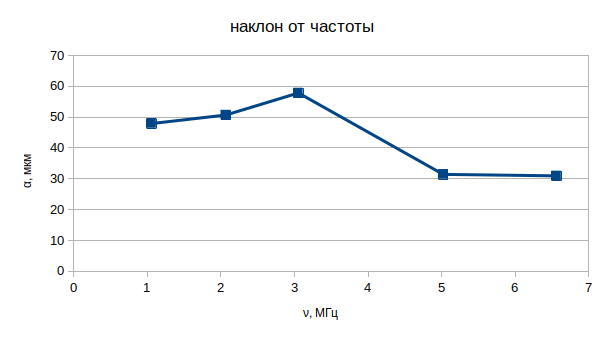
\includegraphics[width=0.9\linewidth]{figures/a(nu).png}
\end{figure}

\begin{enumerate}
	\item Судя по формуле из теории: $\alpha_n \sim \nu_n$, т.е. на интервале
	      $\nu_n \in [1,8]\mega\Hz$ расстояния между максимумами должны были изменятся
	      примерно в 8 раз в ходе эксперимента, чего мы совсем не наблюдали.
	\item Даже если мы ошиблись в порядке или в номерах максимумов, это никак
	      не повлияло бы на тот факт, что у нас $\alpha_n \not\sim \nu_n$. \\
	      Также $\alpha_n$ значительно скачет с частотой ($58 \to 31$),
	      что делу не помогает.
	\item Возможно установление стоячей волны с определенной частотой в емкости
	      с водой это слишком сложная задача. Что если емкость (которая также
	      прямоугольный волновод) резонирует только с частотой $\nu_1 \approx 1
		      \mega\Hz$? Это объясняло бы, почему д.к. не сильно менялась от частоты.
	      Но это лишь догадки.
	\item По поводу второй части, возможно дифракционный максимум был слишком ярким
	      и стоило уменьшить щель. Но, кажется, мы и это пробовали. Казалось бы, что
	      может пойти не так, если мы просто пыаемся загородить луч света проволкой?
\end{enumerate}

\end{document}
